\documentclass[12pt]{report}
\usepackage[utf8]{inputenc}
\usepackage[russian]{babel}
\linespread{1.5}
%\usepackage[14pt]{extsizes}
\usepackage{listings}
\usepackage{float}
\usepackage{graphicx}
\usepackage[left=2cm,right=2cm,
    top=2cm,bottom=2cm,bindingoffset=0cm]{geometry}
\usepackage{amsmath,amsfonts,amssymb,amsthm,mathtools} 



% Для листинга кода:
\lstset{ %
language=c++,                 % выбор языка для подсветки (здесь это С++)
basicstyle=\small\sffamily, % размер и начертание шрифта для подсветки кода
numbers=left,               % где поставить нумерацию строк (слева\справа)
numberstyle=\tiny,           % размер шрифта для номеров строк
stepnumber=1,                   % размер шага между двумя номерами строк
numbersep=5pt,                % как далеко отстоят номера строк от подсвечиваемого кода
showspaces=false,            % показывать или нет пробелы специальными отступами
showstringspaces=false,      % показывать или нет пробелы в строках
showtabs=false,             % показывать или нет табуляцию в строках
frame=single,              % рисовать рамку вокруг кода
tabsize=2,                 % размер табуляции по умолчанию равен 2 пробелам
captionpos=t,              % позиция заголовка вверху [t] или внизу [b] 
breaklines=true,           % автоматически переносить строки (да\нет)
breakatwhitespace=false, % переносить строки только если есть пробел
escapeinside={\#*}{*)}   % если нужно добавить комментарии в коде
}

% Для измененных титулов глав:
\usepackage{titlesec, blindtext, color} % подключаем нужные пакеты
\definecolor{gray75}{gray}{0.75} % определяем цвет
\newcommand{\hsp}{\hspace{20pt}} % длина линии в 20pt
% titleformat определяет стиль
\titleformat{\chapter}[hang]{\Huge\bfseries}{\thechapter\hsp\textcolor{gray75}{|}\hsp}{0pt}{\Huge\bfseries}


% plot
\usepackage{pgfplots}
\usepackage{filecontents}
\usetikzlibrary{datavisualization}
\usetikzlibrary{datavisualization.formats.functions}


\begin{document}
%\def\chaptername{} % убирает "Глава"
\begin{titlepage}

	\fontsize{12pt}{12pt}\selectfont
	\noindent \begin{minipage}{0.15\textwidth}
		
\includegraphics[width=\linewidth]{b_logo.png}
	\end{minipage}
	\noindent\begin{minipage}{0.9\textwidth}\centering
		\textbf{Министерство науки и высшего образования Российской Федерации}\\
		\textbf{Федеральное государственное бюджетное образовательное учреждение высшего образования}\\
		\textbf{«Московский государственный технический университет имени Н.Э.~Баумана}\\
		\textbf{(национальный исследовательский университет)»}\\
		\textbf{(МГТУ им. Н.Э.~Баумана)}
	\end{minipage}
	
	\noindent\rule{18cm}{3pt}
	\newline\newline
	\noindent ФАКУЛЬТЕТ $\underline{\textbf{«Информатика и системы управления»}}$ \newline\newline
	\noindent КАФЕДРА $\underline{\textbf{«Программное обеспечение ЭВМ и информационные технологии»}}$\newline\newline\newline\newline
	
	\begin{center}
		\Large\textbf{Отчет по лабораторной работе №5 по курсу <<Анализ алгоритмов>>}
	\end{center}
	\newline\newline 
	\newline
	
	\noindent\textbf{Тема} $\underline{\textbf{Конвейерная обработка~~~~~~~~~~~~~~~~~~~~~~~~~~~}}$\newline\newline
	\noindent\textbf{Студент} $\underline{\textbf{Челядинов И.Д.~~~~~~~~~~~~~~~~~~~~~~~~~~~~~~~~~}}$\newline\newline
	\noindent\textbf{Группа} $\underline{\textbf{ИУ7-53Б~~~~~~~~~~~~~~~~~~~~~~~~~~~~~~~~~~~~~~~~~~~~}}$\newline\newline
	\noindent\textbf{Оценка (баллы)} $\underline{\textbf{~~~~~~~~~~~~~~~~~~~~~~~~~~~~~~~~~~~~~~~~~~}}$\newline\newline
	\noindent\textbf{Преподаватели} $\underline{\textbf{Волкова Л.Л., Строганов Ю.В.}}$\newline
	
	\begin{center}
		\vfill
		Москва~---~\the\year
		~г.
	\end{center}
 \restoregeometry
\end{titlepage}

\tableofcontents

\newpage
\chapter*{Введение}
\addcontentsline{toc}{chapter}{Введение}
Цель работы: создать систему конвейерной обработки.

Задачи данной лабораторной работы:
\begin{enumerate}
        \item спроектировать ПО, реализующего конвейерную обработку;
        \item описать реализацию ПО;
        \item провести тестирование ПО.
\end{enumerate}



\chapter{Аналитическая часть}
В данной части будут рассмотрены главные принципы конвейерной обработки и параллельных вычислений.

\section{Общие сведения о конвейерной обработке}

\parindent=1cm

	\textbf{Конвейер} – машина непрерывного транспорта, предназначенная для перемещения сыпучих, кусковых или штучных грузов.\cite{mednov}
\parindent=1cm

	\textbf{Конвейерное производство} - система поточной организации производства на основе конвейера, при которой оно разделено на простейшие короткие операции, а перемещение деталей осуществляется автоматически. Это такая организация выполнения операций над объектами, при которой весь процесс воздействия разделяется на последовательность стадий с целью повышения производительности путём одновременного независимого выполнения операций над несколькими объектами, проходящими различные стадии. Конвейером также называют средство продвижения объектов между стадиями при такой организации.\cite{wiki} Появилось в 1914 году на производстве Модели-Т на заводе Генри Форда и произвело революцию сначала в автомобилестроении, а потом и во всей промышленности.\cite{ford}

\section{Параллельное программирование}
	\textbf{Параллельные вычисления} — способ организации компьютерных вычислений, при котором программы разрабатываются как набор взаимодействующих вычислительных процессов, работающих параллельно (одновременно). 

При использовании многопроцессорных вычислительных систем с общей памятью обычно предполагается, что имеющиеся в составе системы процессоры обладают равной производительностью, являются равноправными при доступе к общей памяти, и время доступа к памяти является одинаковым (при одновременном доступе нескольких процессоров к одному и тому же элементу памяти очередность и синхронизация доступа обеспечивается на аппаратном уровне). Многопроцессорные системы подобного типа обычно именуются симметричными мультипроцессорами (symmetric multiprocessors, SMP).

Перечисленному выше набору предположений удовлетворяют также активно развиваемые в последнее время многоядерные процессоры, в которых каждое ядро представляет практически независимо функционирующее вычислительное устройство.

Обычный подход при организации вычислений для многопроцессорных вычислительных систем с общей памятью – создание новых параллельных методов на основе обычных последовательных программ, в которых или автоматически компилятором, или непосредственно программистом выделяются участки независимых друг от друга вычислений. Возможности автоматического анализа программ для порождения параллельных вычислений достаточно ограничены, и второй подход является преобладающим. При этом для разработки параллельных программ могут применяться как новые алгоритмические языки, ориентированные на параллельное программирование, так и уже имеющиеся языки, расширенные некоторым набором операторов для параллельных вычислений.

Широко используемый подход состоит и в применении тех или иных библиотек, обеспечивающих определенный программный интерфейс (application programming interface, API) для разработки параллельных программ. В рамках такого подхода наиболее известны Windows Thread API. Однако первый способ применим только для ОС семейства Microsoft Windows, а второй вариант API является достаточно трудоемким для использования и имеет низкоуровневый характер.\cite{Barkalov}

\subsection{Организация взаимодействия параллельных потоков}
	Потоки исполняются в общем адресном пространстве параллельной программы. Как результат, взаимодействие параллельных потоков можно организовать через использование общих данных, являющихся доступными для всех потоков. Наиболее простая ситуация состоит в использовании общих данных только для чтения. В случае же, когда общие данные могут изменяться несколькими потоками, необходимы специальные усилия для организации правильного взаимодействия.

\section{Вывод}
В данном разделе были рассмотрены основы конвейерной обработки, технология параллельного программирования и
организация взаимодействия параллельных потоков.



\chapter{Конструкторская часть}
\textbf{Требования к вводу:}
Количество конвейеров должно быть больше 0.
\newline
\textbf{Требования к программе при параллельной обработке:}
\begin{itemize}
\item Объекты должны последовательно проходить конвейеры в заданном подядке;
\item конвейеры должны работать каждый в своем потоке;
\item до завершения работы конвейер должен ожидать поступления новых элементов.
\end{itemize}

\section{Организация обработки}
На рисунке 2.1 представлена схема организации конвейерных вычислений.
\begin{figure}[H]
	\center{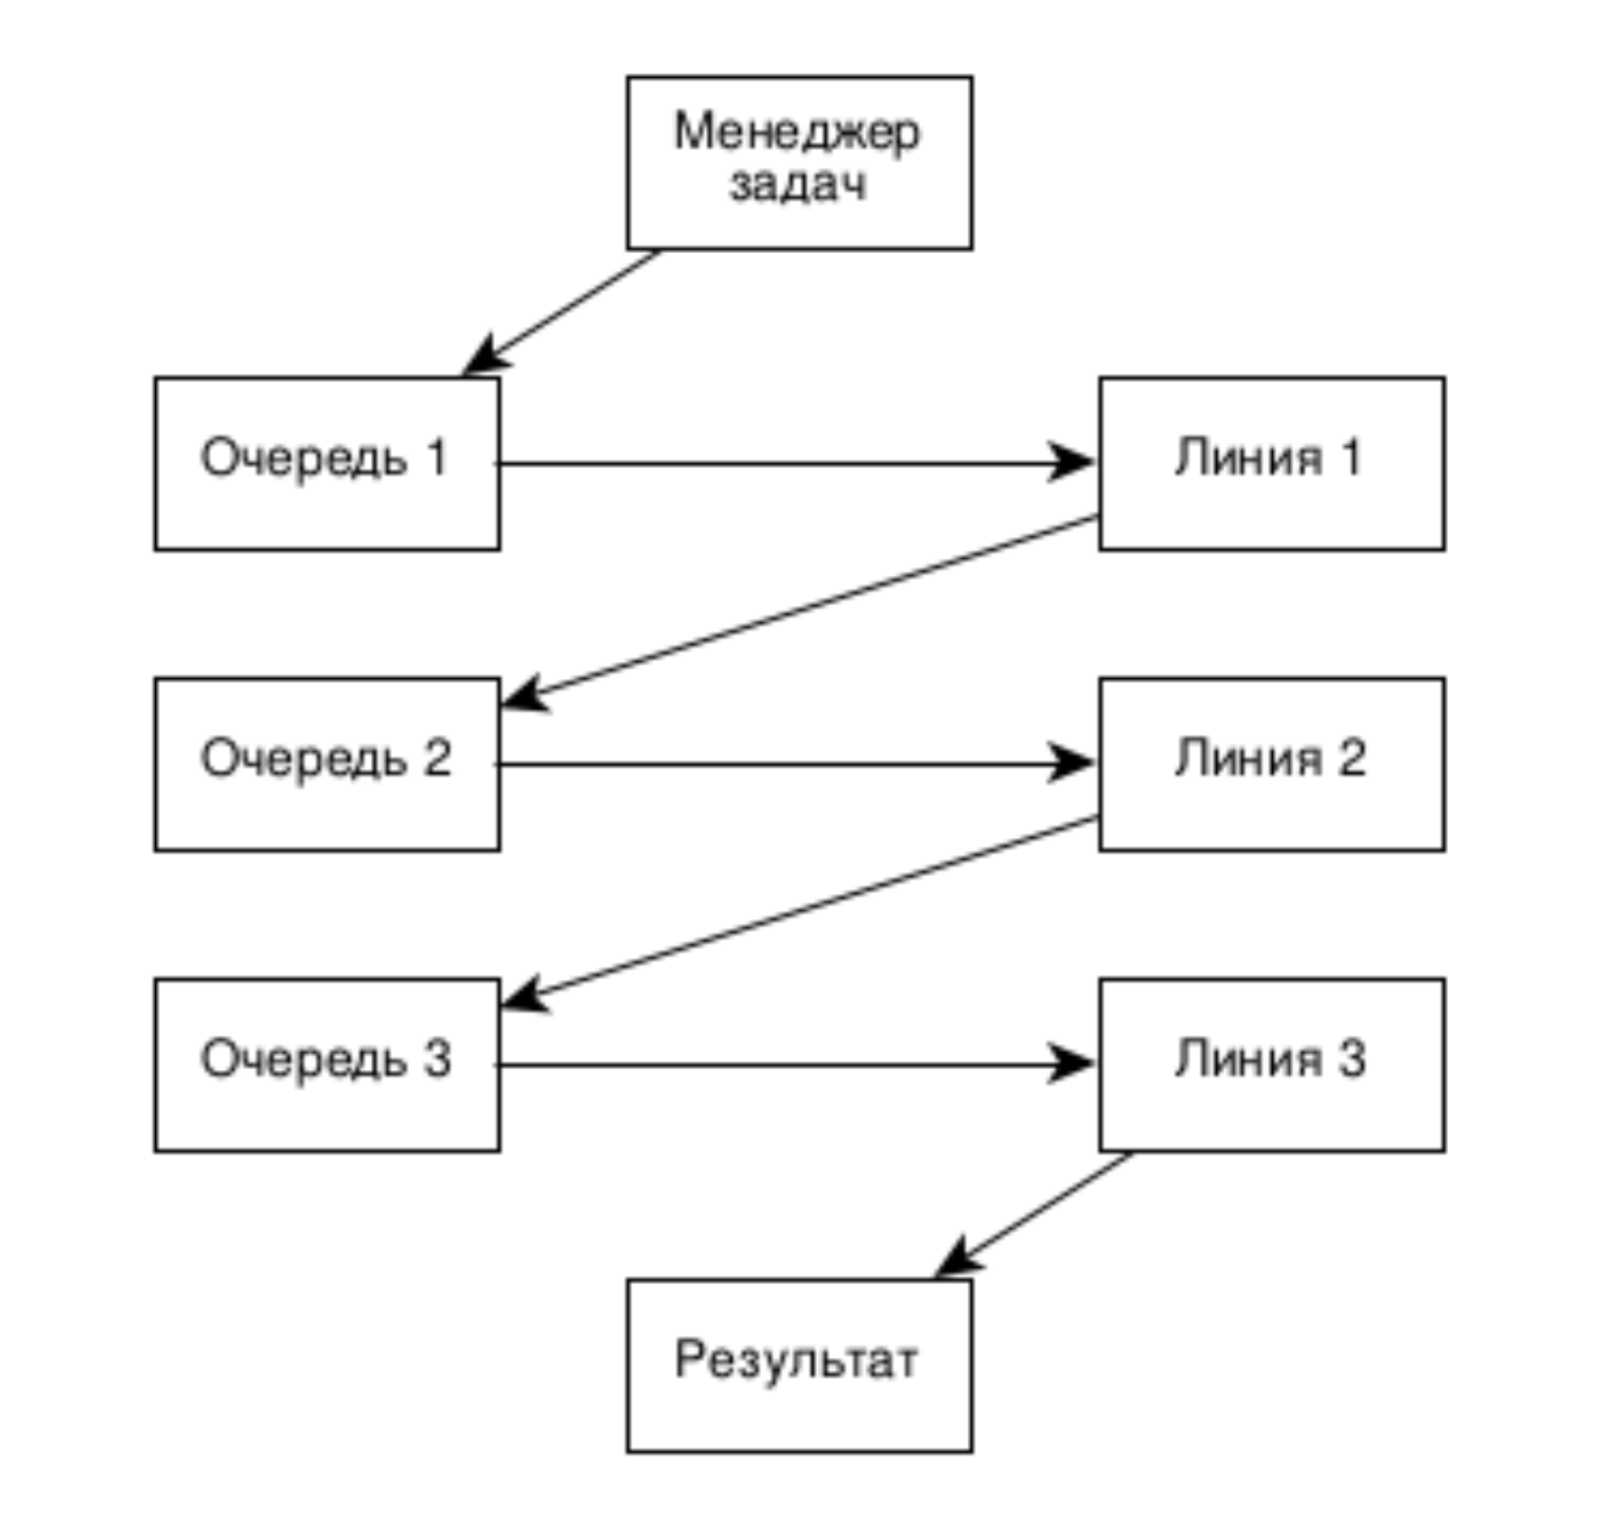
\includegraphics[scale = 0.7]{2.png}}
	\caption{Схема организации конвейерных вычислений}
	\label{fig:v_st}
\end{figure}


\section{Вывод}
В данном разделе была рассмотрена схема организации конвейерной обработки.

 

\chapter{Технологическая часть}
Замеры времени были произведены на: Intel(R) Core(TM) i5 с тактовой частотой 1.4GHz, 4 ядра, 8 логических процессоров.

\section{Выбор ЯП}
В качестве языка программирования был выбран Golang  так как этот
язык поддерживает управление потоками на уровне ОС(незеленые потоки).\cite{Microsoft} Средой разработки Visual Studio Code. 
Время работы алгоритмов было замерено с помощью класса Time. Многопоточное программирование было
реализовано с помощью встроенной функции языка Golang "goroutine".

\section{Листинг кода алгоритмов}
В листинге 3.1 представлен модуль программы, в котором запускаются потоки.
\begin{lstlisting}[label=some-code,caption=Модуль запуска конвейера]
func Сonveyor(n int) *Queue {
	bread := make(chan *Person, 1)
	s := make(chan *Person, 1)
	t := make(chan *Person, 1)

	q := createQueue(n)
	for i := 1; i <= n; i++ {
		go produce(bread)
	}
	for i := 1; i <= n; i++ {
		go consume(bread, s)
	}
	for i := 1; i <= n; i++ {
		go ret(s, t)
	}
	for i := 1; i <= n; i++ {
		time.Sleep(100 * time.Microsecond)
		el := <-t
		q.push(el)
	}
	return q
}
\end{lstlisting}
В листинге 3.2 представлен первый уровень конвейера.
\begin{lstlisting}[label=some-code,caption=Первый уровень конвейера]
func produce(ch chan<- *Person) {
	var pers Person
	pers.email = gofakeit.Email()
	pers.startEmail = time.Now()
	ch <- (&pers)
}
\end{lstlisting}

В листинге 3.2 представлен второй уровень конвейера.
\begin{lstlisting}[label=some-code,caption=Второй уровень конвейера]
func consume(ch chan *Person, ch1 chan *Person) {
	pers := <-ch
	pers.name = gofakeit.Name()
	pers.startName = time.Now()
	ch1 <- pers
}
\end{lstlisting}
В листинге 3.2 представлен третий уровень конвейера.
\begin{lstlisting}[label=some-code,caption=Третий уровень конвейера]
func ret(ch chan *Person, ch1 chan *Person) {
	pers := <-ch
	pers.phone = gofakeit.Phone()
	pers.startNumber = time.Now()
	ch1 <- pers
	// q.push(pers)
}
\end{lstlisting}

\section{Вывод}
В данном разделе были рассмотрены основные сведения о модулях программы, листинг кода.


\chapter{Исследовательская часть}

\section{Пример работы программы}

На рисунке 4.1 представлена работа программы (лог операций конвейера):
\begin{figure}[h]
	\center{\includegraphics[scale = 0.7]{hui.png}}
	\caption{Лог работы конвейерной обработки}
	\label{fig:v_st}
\end{figure}
\begin{center}

\end{center}


На графиках видно, что конвейерная обработка с параллельными потоками в 2.5 раза быстрее чем такая же линейная с захватом переменных.
Если же убрать ненужные захваты переменных (т.к. все действия происходят линейно, не может быть одновременного обращения к одной области памяти), то это будет работать в 2.5 раза быстрее, чем параллельный.

\section{Тестирование}
Тестирование произовдилось с помощью встроенной системы тестирования языка Golang "Benchmark".


На рисунке 4.2 представлены результаты работы бенчмарков:
\begin{figure}[h]
	\center{\includegraphics[scale = 0.7]{pizda.png}}
	\caption{Лог работы конвейерной обработки}
	\label{fig:v_st}
\end{figure}




\section{Вывод}
По результатам исследования, ассинхронные конвейерные вычисления позволяют сэкономить время в задачах, где необходима обработка большого объема данных за малый промежуток времени. Конвейерную обработку нет смысла применять для задач, занимающих мало времени, т.к. в этом случее большая часть времени
потратится на ожидание доступа к переменной, дополнительных проверок.
Тестирование показало, что конвейерная обработка реализована правильно.

\chapter*{Заключение}
\addcontentsline{toc}{chapter}{Заключение}
В ходе лабораторной работы я изучил возможности применения параллельных вычислений и конвейерной обработки и использовал такой подход на практике. 

Конвейерная обработка позволяет сильно ускорить программу, если требуется обработать набор из однотипных данных, причем алгоритм обработки должен быть разбиваем на стадии. Однако от конвейерной обработки не будет смысла, если одна из стадий намного более трудоемкая, чем остальные, так как производительность всей программы будет упираться в производительность этой самой стадии, и разницы между обычной обработкой и конвейерной не будет, только добавятся накладные вычисления, связанные с диспетчеризацией потоков. В таком случае можно либо разбить трудоемкую стадию на набор менее трудоемких, либо выбрать другой алгоритм, либо отказаться от конвейерной обработки.

\addcontentsline{toc}{chapter}{Список литературы}
 \begin{thebibliography}{3}
\bibitem{mednov} Меднов В.П., Бондаренко Е.П. Транспортные, распределительные и рабочие конвейеры. М., 1970.
\bibitem{wiki} Конвейерное производство[Электронный ресурс] - режим доступа https:/ё/dic.academic.ru/dic.nsf/ruwiki/1526795
\bibitem{ford} Koнвeйepный meтoд пpoизвoдcтвa Гeнpи Фopдa[Электронный ресурс] - режим доступа https://popecon.ru/305-konveiernyi-metod-proizvodstva-genri-forda.html
\bibitem{Barkalov}
Константин Баркалов, Владимир Воеводин, Виктор Гергель. Intel Parallel Programming [Электронный ресурс], - режим доступа https://www.intuit.ru/studies/courses/4447/983/lecture/14925
\bibitem{Microsoft}
Руководство по языку Golang[Электронный ресурс], - режим доступа: 
https://golang.org
\end{thebibliography}


\end{document}